\subsection{\bt{Validity under data changes}{数据变化下的有效性}}
\label{sec:validity}
\bi{\emph{Library replay (Q1).} An earlier round of the end-to-end protocol of Section~\ref{sec:scenarios} with three LLMs (DeepSeek V4.1 Flash, GLM-5.3, and GLM-5.3 Flash) yields \RpLibs\ learned libraries of 3--8 admitted definitions, \RpDefs\ in all. We replay every library under every method on the same data: each of the \RpChanges\ changes of Figure~\ref{fig:scenarios} is applied from the same initial snapshot, and every affected scored question is answered with the canonical SQL of the revision the method serves, \RpCondN\ questions per method. This isolates maintenance from learning and agent behavior. A question is \emph{correct}, \emph{wrong}, or \emph{invalidated}; an invalidation is \emph{correct} if the unmaintained definition would also have answered wrongly, and \emph{false} otherwise.}
{\emph{定义库回放（Q1）。}第~\ref{sec:scenarios} 节的端到端流程此前用三个大模型（DeepSeek V4.1 Flash、GLM-5.3、GLM-5.3 Flash）运行的一轮得到 \RpLibs\ 个学到的定义库，各含 3--8 个已准入定义，共 \RpDefs\ 个。我们在同一份数据上用每种方法回放每个库：图~\ref{fig:scenarios} 的 \RpChanges\ 种变化都从同一初始快照施加，每道受影响的计分题用该方法提供的修订的规范 SQL 作答，每种方法 \RpCondN\ 道题。这把维护与学习、与智能体行为隔离开。每道题的结果为\emph{答对}、\emph{答错}或\emph{失效}；若未经维护的定义同样会答错，则该失效为\emph{正确失效}，否则为\emph{误失效}。}

\begin{figure}[t]
\centering
% Vector drawing generated by tools/figures/build.py; rerun it after changing the figure.
\ifbilingual
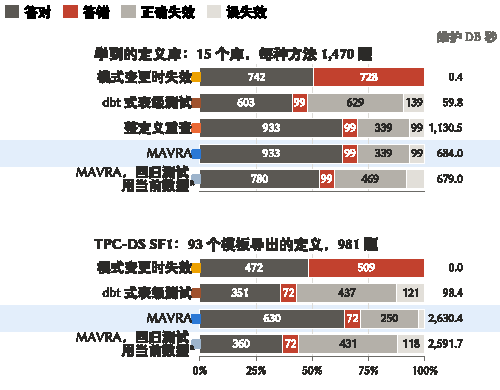
\includegraphics[width=\linewidth]{figures/replay-outcomes-zh}
\else
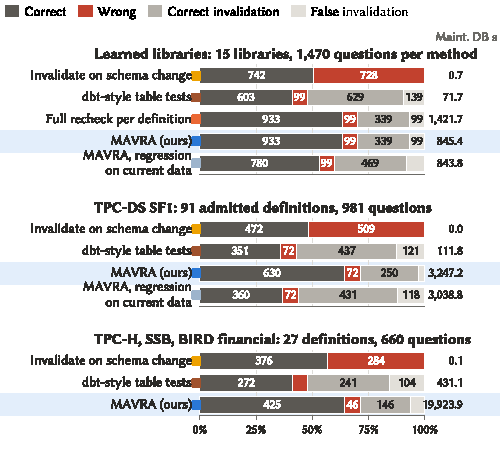
\includegraphics[width=\linewidth]{figures/replay-outcomes}
\fi
\caption{\bt{Library replay: \RpLibs\ learned libraries under \RpChanges\ data changes, \RpCondN\ scored questions per method, split by outcome; numbers at the right are maintenance database seconds. Every method uses the agent's own learning SQL for admission and as the G8 reference. Revalidation methods serve wrong answers only under the unit change, which no condition covers. $^a$Without relearning. $^b$G8 reference is the benchmark's gold SQL, which filters on the distinguishing columns in advance.}{定义库回放：\RpLibs\ 个学到的定义库，\RpChanges\ 种数据变化，每种方法 \RpCondN\ 道计分题，按结果划分；右侧数字为维护数据库秒数。所有方法都以智能体自己的学习 SQL 准入，并以它作 G8 的对照。各重验证方法只在任何条件都不覆盖的单位变化下提供错误答案。$^a$不重新学习。$^b$G8 对照为基准的标准答案 SQL，它预先带有区分列过滤。}}
\label{fig:replay}
\Description{Horizontal stacked bars, one per method, splitting 1,470 scored questions into correct, wrong, correct invalidation, and false invalidation. Schema-change invalidation answers 742 correctly and 728 wrongly; table tests 603 correct, 99 wrong, 629 correct invalidations; invalidate-on-write answers nothing; definition-level, the check-result cache, and MAVRA each answer 780 correctly and 99 wrongly with 469 correct invalidations; MAVRA with the gold SQL answers 933 correctly and 99 wrongly. Maintenance database time ranges from 0.4 s for invalidate-on-write to 1,114 s for definition-level, with MAVRA at 674 s.}
\end{figure}


\bi{Every revalidation method serves wrong answers only under the unit change, which no condition covers, whereas invalidation on schema change serves \RpSchemaWrongModeled\ wrong answers under the covered changes (Figure~\ref{fig:replay}). \system, the full recheck per definition, and the query cache give the same outcome on every question (\RpSameCondDef\%), so their end-to-end differences come from what agents learned. False invalidations are conservative: they arise mostly for return rate, whose ratio can stay right while its grain is broken.}
{各重验证方法只在任何条件都不覆盖的单位变化下给出错误答案，而只在模式变更时失效在条件覆盖的变化下给出 \RpSchemaWrongModeled\ 个错误答案（图~\ref{fig:replay}）。\system、整定义重查与查询缓存在每道题上的结果都相同（\RpSameCondDef\%），因此它们在端到端上的差别来自智能体学到的内容。误失效是保守的：它主要出现在退货率上，粒度已被破坏而比率碰巧仍然正确。}

\bi{\emph{dbt-style table tests} (key uniqueness per table, referential tests on date and item keys, every definition on a failing table invalidated) serve no wrong answer under the covered changes (\RpTableWrongModeled) but cannot repair: they answer \RpTableCorrect\ questions against \RpCondCorrect, and acting on tables rather than definitions gives \RpTableUnneeded\ false invalidations against \RpCondUnneeded.}
{\emph{dbt 式表级测试}（每张表的键唯一性、日期键与商品键的引用测试，测试失败的表上的定义全部失效）在条件覆盖的变化下不给出错误答案（\RpTableWrongModeled），但不能修复：它答对 \RpTableCorrect\ 题，\system\ 答对 \RpCondCorrect\ 题；按表而不是按定义行动带来 \RpTableUnneeded\ 次误失效，\system\ 为 \RpCondUnneeded\ 次。}

\bi{\emph{Real TPC-DS data.} The same replay runs on TPC-DS at scale factor 1 (2.9 million store-sales rows) with a library that was not written for this paper: the \TrDefs\ definitions that the derivation of Section~\ref{sec:alternatives} extracts from the 99 query templates and that the structured implementation can express, of which \TrSeeded\ pass admission; each definition's canonical SQL plays the agent's learning SQL. The middle panel of Figure~\ref{fig:replay} matches the synthetic fixture: \system\ serves no wrong answer under the covered changes, repairs every affected definition under status-change rows, restatements, and SCD Type 2 (\TrCondRepairedTasks\ questions answered through a repair), and invalidates the definitions under duplicate loads, the date-key format change, and the backup copy; invalidation on schema change serves \TrSchemaWrongModeled\ wrong answers, and table tests repair nothing.}
{\emph{真实 TPC-DS 数据。}同一回放也在规模因子 1 的 TPC-DS（290 万行门店销售）上运行，定义库不是为本文编写的：第~\ref{sec:alternatives} 节的推导从 99 个查询模板中提取、且结构化实现能够表达的 \TrDefs\ 个定义，其中 \TrSeeded\ 个通过准入；每个定义的规范 SQL 充当智能体的学习 SQL。图~\ref{fig:replay} 中间的面板与合成数据一致：\system\ 在条件覆盖的变化下不给出错误答案，在状态流水、更正保留旧行与缓慢变化维（类型 2）下修复了每一个受影响的定义（\TrCondRepairedTasks\ 道题经修复后作答），在重复加载、日期键格式变化与备份副本下使定义失效；只在模式变更时失效给出 \TrSchemaWrongModeled\ 个错误答案，表级测试一个也不能修复。}

\bi{\emph{Three more schemas.} On TPC-H, SSB, and BIRD financial, \GnKept\ of the \GnDerived\ definitions derived from the benchmarks' queries have a nonzero learning answer, and all pass admission (bottom panel of Figure~\ref{fig:replay}). The pattern is that of TPC-DS, with \GnCondRepairedTasks\ questions answered through a repair; outside the unit change \system\ serves \GnCondWrongModeled\ wrong answers, all from one TPC-H definition whose filter reads a ship date that the date-key change empties and no condition reads (Section~\ref{sec:sufficiency}), against \GnSchemaWrongModeled\ for invalidation on schema change. SSB's yyyymmdd keys skip numbers between months, so date-key contiguity fails in \GnSsbContigBad\ of \GnSsbMonths\ months and the key-range rule is refused there.}
{\emph{另外三种模式。}在 TPC-H、SSB 与 BIRD financial 上，从基准查询导出的 \GnDerived\ 个定义中有 \GnKept\ 个的学习题答案非空、非零，全部通过准入（图~\ref{fig:replay} 最下面的面板）。结果与 TPC-DS 相同，\GnCondRepairedTasks\ 题经修复作答；单位变化之外 \system\ 给出 \GnCondWrongModeled\ 个错误答案，全部来自 TPC-H 的同一个定义：其过滤读取发货日期，日期键变化清空了这一列，而没有条件读它（第~\ref{sec:sufficiency} 节），只在模式变更时失效给出 \GnSchemaWrongModeled\ 个。SSB 的 yyyymmdd 日期键在月与月之间跳号，\GnSsbMonths\ 个月中有 \GnSsbContigBad\ 个月不满足日期键连续，键范围改写因此在 SSB 上被拒绝。}
